\section*{§ 12. Фильтрация с учетом слабой сжимаемости жидкости и пористого скелета}
% Источник: Leontiev-2017.pdf; печатная страница: 70; страница файла: 70
\topic{Упругий режим фильтрации}
В отличие от газов, которые могут в разы менять свой объем, капельные жидкости (вода, нефть) являются \textit{слабосжимаемыми} веществами, у которых в промысловых условиях относительное изменение объема составляет доли процента. Поэтому, во-первых, при изучении эффектов сжимаемости на фильтрацию жидкостей нужно одновременно учитывать и сжимаемость пористого скелета и, во-вторых, учет этих изменений можно проводить в линейном приближении.

В соответствии с этим к системе, состоящей из уравнения неразрывности и закона Дарси:
\[
(m\rho)'_t+\Div(\rho\boldsymbol u)=0,\qquad \boldsymbol u=-\frac{k}{\mu}\grad p,
\]
добавляются \textit{линейные} соотношения, определяющие изотермические зависимости плотности $\rho$, пористости $m$, проницаемости $k$ и вязкости $\mu$ от возмущения давления жидкости в порах по сравнению с некоторым начальным состоянием $p_0$\footnote{Тем самым мы предполагаем деформации жидкости и пористого скелета \textit{обратимыми} (упругими), в связи с чем о процессах, при которых эта теория справедлива, говорят как об \textit{упругом режиме фильтрации}.}:
\begin{equation}\begin{aligned}
\rho(p)&=\rho_0\cdot\left(1+\frac{p-p_0}{K_\rho}\right),&m(p)&=m_0\cdot\left(1+\frac{p-p_0}{K_m}\right),\\
k(p)&=k_0\cdot\left(1+\frac{p-p_0}{K_k}\right),&\mu(p)&=\mu_0\cdot\left(1+\frac{p-p_0}{K_\mu}\right),
\end{aligned}\tag{12.1}\label{q8:eq-12-1}\end{equation}
где величины $\rho_0,m_0,k_0,\mu_0$ относятся к невозмущенному состоянию, а константы $K_\rho,K_m,K_k,K_\mu$ являются упругими модулями\footnote{Например, при $10^\circ$C для воды $K_\rho\approx2\cdot10^4$ атм, $K_\mu\approx-2\cdot10^4$ атм; отрицательное значение $K_\mu$ соответствует падению вязкости воды при не очень большом повышении давления.}, которые характеризуют изменение свойств пористой среды и жидкости при всестороннем сжатии и по порядку величины много больше характерных возмущений давления: $(p-p_0)/K\ll1$.

% Источник: Leontiev-2017.pdf; печатная страница: 71; страница файла: 71
\setcounter{footnote}{0}
Как и в случае фильтрации газа (§ 11), мы подставим закон Дарси в уравнение неразрывности:
\[
\frac{\partial(m(p)\rho(p))}{\partial t}=\Div\left(\frac{\rho(p)k(p)}{\mu(p)}\grad p\right),
\]
что после преобразований дает
\[
\rho m\left(\frac{m'_p}{m}+\frac{\rho'_p}{\rho}\right)p'_t=\frac{\rho k}{\mu}\left\{\left(\frac{\rho'_p}{\rho}+\frac{k'_p}{k}+\frac{(1/\mu)'_p}{1/\mu}\right)|\grad p|^2+\Delta p\right\},
\]
и, поскольку мы хотим получить уравнения для \textit{малых возмущений}, упростим коэффициенты при производных от давления: вместо значений $k,\mu,\rho$ и $m$ возьмем их невозмущенные значения $k_0,\mu_0,\rho_0$ и $m_0$, а при вычислении производных воспользуемся линейными уравнениями состояния \eqref{q8:eq-12-1}, например:
\[
\frac{\rho'_p}{\rho}\approx\frac{1}{K_\rho},\qquad \frac{(1/\mu)'_p}{1/\mu}\approx-\frac{1}{K_\mu}.
\]
В результате получится уравнение с постоянными коэффициентами, в котором дополнительно можно отбросить нелинейное слагаемое\footnote{Зачеркнутый член имеет порядок $(p-p_0)^2/(KL^2)$, где $L$ --- характерный размер задачи, а оператор Лапласа порядка $(p-p_0)/L^2$, так что отношение этих членов порядка $(p-p_0)/K\ll1$.}:
\[
\rho_0m_0\left(\frac{1}{K_m}+\frac{1}{K_\rho}\right)p'_t=\frac{\rho_0k_0}{\mu_0}\left\{\cancel{\left(\frac{1}{K_\rho}+\frac{1}{K_k}-\frac{1}{K_\mu}\right)|\grad p|^2}+\Delta p\right\},
\]
что в итоге дает \textit{уравнение пьезопроводности}\footnote{Название (от греч. $\pi\iota\varepsilon\zeta\omega$ --- «давлю») дано по аналогии с названием уравнения теплопроводности, совпадающего по форме с (12.2).}, полученное рядом исследователей в 1930--40-х гг. [11,17]:
\begin{equation}
p'_t=\varkappa\Delta p,\qquad \varkappa=\frac{k_0}{m_0\mu_0}\left(\frac{1}{K_\rho}+\frac{1}{K_m}\right)^{-1}=\mathrm{const},\tag{12.2}\label{q8:eq-12-2}
\end{equation}
где $\varkappa$ --- \textit{коэффициент пьезопроводности}. Граничные условия для уравнения \eqref{q8:eq-12-2} ставятся аналогично условиям при изотермической фильтрации газа (стр. 67).

% Источник: Leontiev-2017.pdf; печатная страница: 72; страница файла: 72
\setcounter{footnote}{0}
Коэффициент пьезопроводности одновременно учитывает сжимаемость жидкости и пористого скелета. Отметим, что в промысловых условиях встречаются ситуации, когда фильтрующаяся жидкость содержит пузырьки газа (например, газ, растворенный в жидкости, может выделяться при понижении давления). Это приводит к увеличению средней сжимаемости флюида и, как следствие, к резкому снижению эффективного коэффициента пьезопроводности $\varkappa$.

\topic{Распространение волны давления в пласте}
Рассмотрим одномерную задачу движении плоской волны давления в полубесконечном пористом пласте. Предположим, что начальное давление флюида в пласте постоянно, а в нулевой момент времени давление на границе пласта \textit{скачком} повышается на постоянную величину $\delta p$ и далее все время поддерживается на этом уровне. Считая для простоты начальное давление нулевым: $p_0=0$\footnote{В уравнение пьезопроводности входят только производные от давления.} и направляя ось $Ox$ вдоль пласта, получим задачу
\begin{equation}
p'_t=\varkappa p''_{xx},\quad p(x,0)=0,\quad p(0,t)=\delta p,\quad \lim_{x\to\infty}p(x,t)=0\tag{12.3}\label{q8:eq-12-3}
\end{equation}
(начало координат выбрано на границе пласта). Решение задачи автомодельно и, в соответствии с $\pi$-теоремой, имеет вид
\[
p=p(x,t,\varkappa,\delta p)=\delta p\cdot f(\xi),\qquad \xi=\frac{x}{\sqrt{\varkappa t}},
\]
что сводит \eqref{q8:eq-12-3} к краевой задаче для обыкновенного дифференциального уравнения
\[
2f''(\xi)+\xi f'(\xi)=0,\quad f(0)=1,\quad f(\infty)=0,
\]
решение которой выражается через функцию ошибок (рис. \ref{q8:fig-27} \textit{а}):
\[
f(\xi)=1-\operatorname{erf}(\xi/2),\qquad \operatorname{erf}x=\frac{2}{\sqrt\pi}\int_0^x\exp(-\alpha^2)\,d\alpha.
\]
В размерных переменных распределение давления дается выражением
\[
p(x,t)=\delta p\cdot\left(1-\operatorname{erf}\left(\frac{x}{2\sqrt{\varkappa t}}\right)\right);
\]
% Источник: Leontiev-2017.pdf; печатная страница: 73; страница файла: 73
качественный вид пространственного распределения давления для трех моментов времени $t_1<t_2<t_3$ показан на рис. \ref{q8:fig-27} \textit{б}.
\setcounter{figure}{26}
\begin{figure}[H]\centering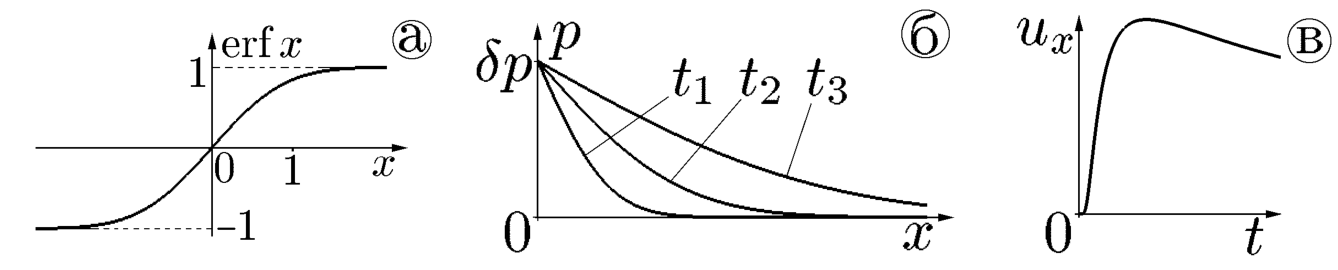
\includegraphics[width=.95\linewidth]{figures/fig-27.png}\caption{}\label{q8:fig-27}\end{figure}
Скорость фильтрации, которая находится с помощью закона Дарси:
\[\begin{aligned}
u_x(x,t)&=-\frac{k(p(x,t))}{\mu(p(x,t))}p'_x(x,t)\approx-\frac{k_0}{\mu_0}p'_x(x,t)=\\
&=\frac{k_0\delta p}{\mu_0}\frac{1}{\sqrt{\pi\varkappa t}}\exp\left(-\frac{x^2}{4\varkappa t}\right),
\end{aligned}\]
в каждой фиксированной внутренней точке пласта с течением времени сначала возрастает от нулевого значения до некоторого максимального, а затем постепенно падает до нуля при $t\to\infty$ (рис. \ref{q8:fig-27} \textit{в}).

С помощью этого решения несложно оценить характерное время $\tau$ переходного процесса в упругом режиме: $\tau\sim L^2/\varkappa$. При характерных параметрах $K\sim10^4$ атм, $k\sim10^{-8}$ см$^2$, $\mu\sim10^{-2}$ г/(см$\cdot$с), $m\sim1$ получим $\varkappa\sim1$ м$^2$/с, и если $L\sim10$ м, то $\tau\sim1$ мин, а при $L\sim10^3$ м $\tau\sim10$ сут.

\topic{Пуск скважины с постоянным дебитом}
\setcounter{footnote}{0}
В качестве второго примера использования уравнения пьезопроводности рассмотрим автомодельную задачу о пуске скважины с постоянным дебитом\footnote{Деби́т (франц. débit --- «расход» от лат. debitum --- «долг») --- объемный расход (колодца, скважины). Это название не следует путать с бухгалтерским термином \textit{де́бет}, восходящим к тому же латинскому корню, что и слово \textit{деби́т}.}.

Пусть в тонкий однородный пласт, в котором первоначально находилась покоящаяся жидкость с постоянным давлением, в некоторый момент времени начинается закачка жидкости с постоянным объемным расходом $Q$ (на единицу толщины пласта) через тонкую скважину. Полагая, как и раньше, начальное давление нулевым и пренебрегая толщиной скважины, получим систему для нахождения распределения давления $p(r,t)$, где $r$ ---
% Источник: Leontiev-2017.pdf; печатная страница: 74; страница файла: 74
расстояние до скважины:
\begin{equation}\begin{gathered}
p'_t=\frac{\varkappa}{r}(rp'_r)'_r,\quad p(r,0)=0,\\
\lim_{r\to\infty}p(r,t)=0,\quad Q=\lim_{r\to0}\left(-2\pi r\frac{k_0}{\mu_0}\frac{\partial p}{\partial r}\right).
\end{gathered}\tag{12.4}\label{q8:eq-12-4}\end{equation}
С учетом того, что параметры $Q,\mu_0$ и $k_0$ входят в постановку задачи \eqref{q8:eq-12-4} только в комбинации $Q\mu_0/k_0$, вид зависимости давления от параметров задачи легко находится с помощью $\pi$-теоремы:
\[
p=p(r,t,\varkappa,Q\mu_0/k_0)=\frac{Q\mu_0}{k_0}f(\xi),\qquad\xi=\frac{r}{\sqrt{\varkappa t}},
\]
так что \eqref{q8:eq-12-4} сводится к краевой задаче
\[
-f'(\xi)(1+\xi^2/2)=\xi f''(\xi),\quad f(\infty)=0,\quad\lim_{\xi\to0}(\xi f'(\xi))=-\frac{1}{2\pi},
\]
решение которой имеет вид
\begin{equation}
f(\xi)=-\frac{1}{4\pi}\operatorname{Ei}\left(-\frac{\xi^2}{4}\right),\tag{12.5}\label{q8:eq-12-5}
\end{equation}
где $\operatorname{Ei}$ --- интегральная показательная функция (рис. \ref{q8:fig-28} \textit{а}):
\[
\operatorname{Ei}x=\int_{-\infty}^x\frac{\exp\zeta}{\zeta}\,d\zeta,\quad x<0.
\]
Отсюда находятся распределения давления и скорости фильтрации:
\begin{equation}\begin{aligned}
p(r,t)&=-\frac{Q\mu_0}{4\pi k_0}\operatorname{Ei}\left(-\frac{r^2}{4\varkappa t}\right),&u_r(r,t)&=\frac{Q}{2\pi r}\exp\left(-\frac{r^2}{4\varkappa t}\right).
\end{aligned}\tag{12.6}\label{q8:eq-12-6}\end{equation}
Качественный вид пространственного распределения давления $p(r)$ при $Q>0$ (закачка в пласт) и при $Q<0$ (откачка из пласта или остановка работающей скважины) показан на рис. \ref{q8:fig-28} \textit{б}.

% Источник: Leontiev-2017.pdf; печатная страница: 75; страница файла: 75
\begin{figure}[H]\centering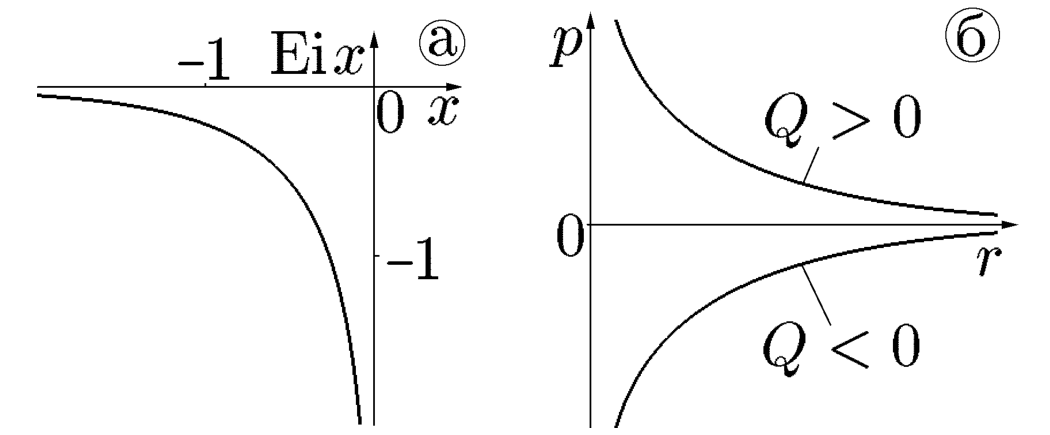
\includegraphics[width=.8\linewidth]{figures/fig-28.png}\caption{}\label{q8:fig-28}\end{figure}
В фиксированной точке пласта $r=r_0$ с течением времени давление возрастает от нулевого значения до бесконечности (рис. \ref{q8:fig-29} \textit{а}), а скорость фильтрации за время порядка $\tau\sim r_0^2/\varkappa$ становится практически постоянной, увеличиваясь от нуля до конечного асимптотического значения $Q/(2\pi r_0)$. При $r_0\sim10^{-1}$ м, что соответствует радиусу реальных скважин, расход через поверхность $r=r_0$ практически мгновенно становится постоянным ($\tau\sim10^{-2}$ с), поэтому это решение, несмотря на формальное обращение в бесконечность скорости фильтрации и давления при $r\to0$, часто используется в гидрогеологических и нефтепромысловых расчетах.

\topic{Об экспериментальном определении параметров пласта}
\setcounter{footnote}{0}
Полученное решение \eqref{q8:eq-12-6} имеет важное значение потому, что оно позволяет определять неизвестные параметры пласта по экспериментальным временны́м зависимостям $p(t)$, измеряемым в самой скважине или в соседних измерительных скважинах\footnote{График функции $p(t)$ называют \textit{кривой восстановления давления} (КВД).}.

Например, при больших временах (или вблизи скважины), что соответствует $\xi\ll1$, формулу \eqref{q8:eq-12-5} можно упростить, воспользовавшись первыми двумя членами разложения интегральной показательной функции\footnote{Доказательство см., например, в книге: Фихтенгольц Г. М. Курс дифференциального и интегрального исчисления. Т. II. М.: Наука, 1969.}
\[
\operatorname{Ei}(-x)=C+\ln x+\sum_{k=1}^\infty\frac{(-x)^k}{k!k}=C+\ln x-x+\frac{x^2}{4}-\ldots,\quad x>0,
\]
% Источник: Leontiev-2017.pdf; печатная страница: 76; страница файла: 76
где $C=0{,}577\ldots$ --- постоянная Эйлера--Маскерони, что приводит к асимптотической формуле
\[
p(r_0,t)=\frac{Q\mu_0}{4\pi k_0}\ln\frac{2{,}25\varkappa t}{r_0^2}.
\]
\setcounter{footnote}{0}
На плоскости $(\ln(\varkappa t/r_0^2);p(r_0,t))$ этой зависимости соответствует прямая (пунктирная линия на рис. \ref{q8:fig-29} \textit{б}), к которой стремится действительная зависимость $p(t)$ при $t\to\infty$. Поэтому построив в полулогарифмических координатах экспериментальную зависимость $p(t)$ при известных $r_0$ и $Q\mu_0$ и определив касательную к прямолинейной части графика\footnote{При достаточно больших временах на виде $p(t)$ может сказываться влияние границ пласта.}, можно найти значения $\varkappa$ и $k_0$.
\begin{figure}[H]\centering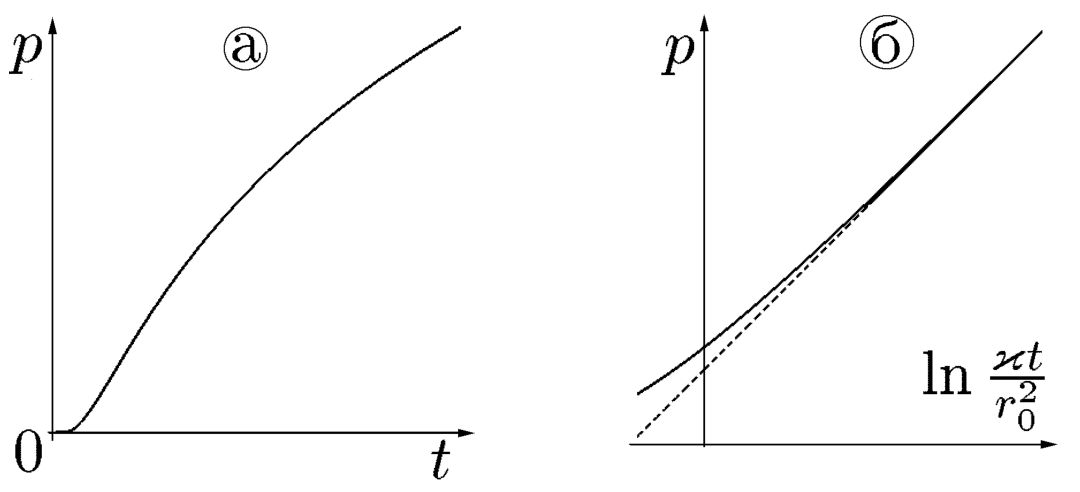
\includegraphics[width=.8\linewidth]{figures/fig-29.png}\caption{}\label{q8:fig-29}\end{figure}
\topic{О связи уравнений Лейбензона, пьезопроводности и Лапласа}
С физической точки зрения три уравнения --- Лейбензона, пьезопроводности и уравнение Лапласа для фильтрации несжимаемой жидкости --- являются уравнениями фильтрации упругой среды в трех характерных случаях, когда сжимаемость является соответственно сильной, слабой и бесконечно малой (отсутствует).

Правая часть уравнения Лейбензона может быть преобразована к виду
\[
\Delta(p^2)=\nabla_i(2p\nabla^i p)=2(|\grad p|^2+p\Delta p),
\]
и при малых возмущениях давления $\delta p$ (по сравнению с фоновым значением $p_0$) квадратом градиента давления можно пренебречь:
\[
\frac{|\grad p|^2}{p\Delta p}\sim\frac{(\delta p/L)^2}{p_0\delta p/L^2}\sim\frac{\delta p}{p_0}\ll1,
\]
% Источник: Leontiev-2017.pdf; печатная страница: 77; страница файла: 77
\setcounter{footnote}{0}
что дает уравнение
\[
p'_t=\frac{kp_0}{m\mu}\Delta p,
\]
являющееся частным видом уравнения пьезопроводности в случае недеформируемого скелета ($K_m\to\infty$)\footnote{Для газа модуль упругости $K_\rho=p_0$, т.к. изотермическое уравнение состояния $\rho=\rho_0p/p_0$ можно записать в виде $\rho=\rho_0(1+(p-p_0)/p_0)$.}.

Далее, при стремлении сжимаемостей флюида и скелета к нулю ($K_\rho\to\infty$, $K_m\to\infty$) коэффициент пьезопроводности $\varkappa$ обращается в бесконечность, и уравнение пьезопроводности переходит в уравнение Лапласа $\Delta p=0$, описывающее фильтрацию несжимаемой жидкости в недеформируемой среде.
